\documentclass[a4]{article}

\usepackage{fullpage}
\usepackage{graphicx}
\usepackage{tikz}
  \usetikzlibrary{arrows}
\usepackage{listings}
\usepackage{theorem}
\usepackage{url}
\usepackage{xspace}
\usepackage{amssymb}
\usepackage{xtab}
\usepackage{todonotes}

%\newcommand{\todo}[1]{{\bf [TODO: }\textit{#1}{\bf ]}}
\newcommand{\remark}[1]{{\bf [RemarkKVH: }\textit{#1}{\bf ]}}
\newcommand{\remarktmb}[1]{{\bf [RemarkTMB: }\textit{#1}{\bf ]}}

\newcommand{\EIS}{\textsf{EIS}\xspace}
\newcommand{\IILang}{\textsf{IILang}\xspace}

\newcommand{\Goal}{\textsc{GOAL}\xspace}
\newcommand{\Jason}{\textsc{Jason}\xspace}
\newcommand{\twoAPL}{\textsc{2APL}\xspace}
\newcommand{\Jadex}{\textsc{Jadex}\xspace}

\newtheorem{example}{Example}





\begin{document}

\title{Environment Interface Standard for Agent-Oriented Programming \\
\textit{Guide for EIS v0.3}
}

\author{Tristan Behrens}
\date{\today}

\maketitle

\section{INTRODUCTION}

This document's intent is 1. to give an overview on how to integrate \EIS with your platform and 2. how to \emph{EISify} your own or third-party environments, that is making it EIS-compatible. This paper is supposed to be a document complemental to the \EIS-javadoc. Things that you will not find
in this document, you will find in the javadoc. For the general motivation behind \EIS please refer
to our technical report\footnote{\url{http://www.in.tu-clausthal.de/fileadmin/homes/techreports/ifi0909behrens.pdf}}.

This document consists of
\begin{enumerate}
\item a \emph{platform guide} that explains how to connect your APL platform to \EIS, and
\item a \emph{interface guide} that explains how to make your environments \EIS-compatible.
\end{enumerate}

\subsection{Building, Installing and Linking}

We can assume that you have already successfully downloaded \EIS from sourceforge. 
To build \EIS you need to have Maven\footnote{\url{http://maven.apache.org/}} installed. Navigate to
the folder that contains the file \texttt{pom.xml} and run this command:
\begin{quote}
\texttt{mvn install}
\end{quote}
This will compile \EIS, run some JUnit tests, bundle the compiled classes into a single jar-file and install it to 
your local Maven-repository. After that you will find the file \texttt{eis-0.3.jar} in the \texttt{target/}-folder.

You can then add this file to the class-path of you project in the traditional way, that is copying and linking by hand. Alternatively, if your project already supports  
Maven you can add \EIS as a dependency to your \texttt{pom.xml}:
\begin{verbatim}
<dependencies>
  <dependency>
    <groupId>apleis</groupId> 
    <artifactId>eis</artifactId> 
    <version>0.3</version> 
    <scope>compile</scope>
  </dependency>
  ...
</dependencies>
\end{verbatim}

\subsection{Interface Meta-Model}

Fig.~\ref{FIGENVMODEL} shows the \EIS interface meta-model. We assume that the overall system consists
of these components:
\begin{itemize}
\item \emph{agents}, 
\item the \emph{platform} that manages and executes agents,
\item the  \emph{environment management system} that facilitates managing the environment,
\item the \emph{agents-entities system} that connects agents to controllable entities,
\item the \emph{environment querying system} that allows for querying the environment-interface for statistics, and
\item the \emph{environment model} that represents the environment itself.
\end{itemize}

\begin{figure}[h]
\begin{center}
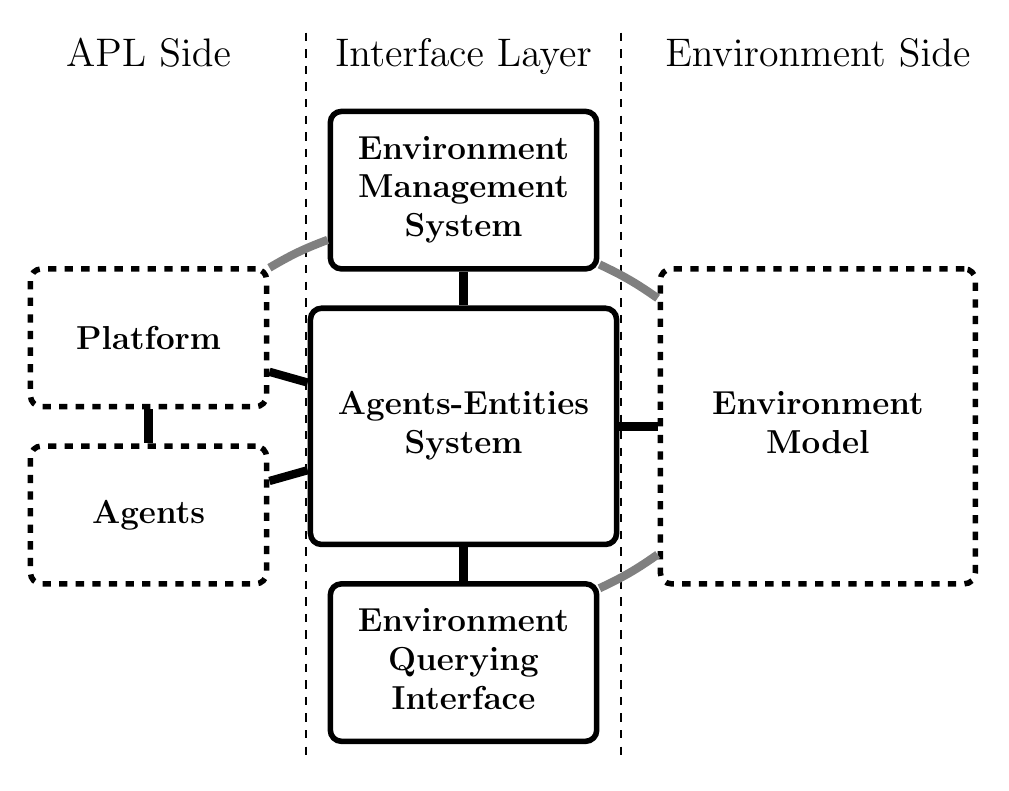
\begin{tikzpicture}[line width=2pt,scale=1]\large
%\draw[-,dashed,line width=1pt] (4,5) to (4,-2.75);
\node(text1) at(0,4.75){\Large APL Side};
\node(text1) at(8.5,4.75){\Large Environment Side};
\node(text1) at(4,4.7){\Large Interface Layer};
\draw[-,dashed,line width=1pt] (2,5) to (2,-4.25);
\draw[-,dashed,line width=1pt] (6,5) to (6,-4.25);

\node[rectangle, draw=black,fill=white,rounded corners, minimum width=3cm, minimum height = 2cm] (envman) at (4,3){\bf \begin{tabular}{ccc}Environment\\Management\\System\end{tabular}};
\node[rectangle, draw=black,fill=white,rounded corners, minimum width=3cm, minimum height = 1.75cm, dashed] (platform) at (0,1.125){\bf Platform};
\node[rectangle, draw=black,fill=white,rounded corners, minimum width=3cm, minimum height = 1.75cm, dashed] (agents) at (0,-1.125){\bf Agents};
\node[rectangle, draw=black,fill=white,rounded corners, minimum width=3cm, minimum height = 3cm] (eis)  at (4,0) {\bf \begin{tabular}{ccc}Agents-Entities\\System\end{tabular}};
\node[rectangle, draw=black,fill=white,rounded corners, minimum width=4cm, minimum height = 4cm, dashed] (env) at (8.5,0){\bf \begin{tabular}{ccc}Environment\\Model\end{tabular}};
\node[rectangle, draw=black,fill=white,rounded corners, minimum width=3cm, minimum height = 2cm] (envquer) at (4,-3){\bf \begin{tabular}{ccc}Environment\\Querying\\Interface\end{tabular}};

\draw[-,line width=3pt] (envman) to (eis);
\draw[-,line width=3pt] (eis) to (agents);
\draw[-,line width=3pt] (platform) to (agents);
\draw[-,line width=3pt] (platform) to (eis);
\draw[-,line width=3pt] (eis) to (env);
\draw[-,line width=3pt,bend right=5,color=gray] (envman) to (platform);
\draw[-,line width=3pt,bend right=5,color=gray] (env) to (envman);
\draw[-,line width=3pt] (eis) to (envquer);
\draw[-,line width=3pt,bend right=5,color=gray] (envquer) to (env);

\end{tikzpicture}
\end{center}
\caption{The interface meta-model. We have three different layers. The platform and its agents live on the APL side. The environment management system, that facilitates the
manipulation of the environments executional state, the
agents-entities system, that connects agents to controllable entities, and the environment-querying system, that allows
for querying the environment and the environment interface for data, all live on the interface layer. And the environment model lives on the environment side.}
\label{FIGENVMODEL}
\end{figure}

\subsection{Interface Intermediate Language}

\todo{Motivation}


The  Interface Intermediate Language (\IILang) consists of 1. \emph{data containers} (e.g. actions and percepts), 2. \emph{parameters}
to those containers, and 3. \emph{environment states} (see Fig.~\ref{FIG:IILANG}). 
Members of the \IILang are stored as abstract syntax trees formed by Java-objects, which can be printed
either in an XML- or in an logic-programming style for the sake of readability.

Parameters are: identifiers, numbers, truth-values, functions over parameters, and lists of parameters.
These are the Java-classes representing parameters:
\begin{itemize}
\item\texttt{eis.iilang.Identifier} represents an identifier,
\item\texttt{eis.iilang.Numeral} represents a number,
\item\texttt{eis.iilang.TruthValue} represents a truth-value,
\item\texttt{eis.iilang.Function} represents a function over parameters, and
\item\texttt{eis.iilang.ParameterList} represents a list of parameters.
\end{itemize}

\begin{figure}[h]\centering
\tikzstyle{node}=[rectangle,draw=black,minimum width =2.5cm,minimum height = 0.75cm]
\begin{tikzpicture}
\node[node] (NA) at (0,-0.75) {\texttt{IILElement}};% at (0,0);
\node[node] (NB1) at (4,1) {\texttt{DataContainer}};
\node[node] (NB2) at (4,-2.5) {\texttt{Parameter}}; 
\node[node] (NC1) at (8,1.5) {\texttt{Action}};
\node[node] (NC2) at (8,0.5) {\texttt{Percept}};
\node[node] (NC3) at (8,-0.5) {\texttt{Identifier}};
\node[node] (NC4) at (8,-1.5) {\texttt{Numeral}};
\node[node] (NC5) at (8,-2.5) {\texttt{TruthValue}};
\node[node] (NC6) at (8,-3.5) {\texttt{ParameterList}};
\node[node] (NC7) at (8,-4.5) {\texttt{Function}};
\draw[-] (NA) to (NB1);
\draw[-] (NA) to (NB2);
\draw[-] (NB1) to (NC1);
\draw[-] (NB1) to (NC2);
\draw[-] (NB2) to (NC3);
\draw[-] (NB2) to (NC4);
\draw[-] (NB2) to (NC5);
\draw[-] (NB2) to (NC6);
\draw[-] (NB2) to (NC7);
\end{tikzpicture}
\caption{The inheritance relation of the IIL-elements. Actions and percepts are data-containers. Each data-container consists of a name and an ordered collection of parameters. Each parameter is either an identifier, a numeral, a list of parameters or a function of parameters.}
\label{FIG:IILANG}
\end{figure}

\todo{Examples!}

Data containers are: actions that are performed by agents,
results of such actions,
percepts that are received by agents, and
events that are sent to agents by the interface.
Furthermore they are:
environment commands that are for example issued to control the execution of the environment, and
events that are sent to notify about changes of the state of execution.

Each of these data containers consist of (1) a name, and (2) a set of parameters.
Here are the respective classes:
\begin{itemize}
\item\texttt{eis.iilang.Action} represents an action.
\item\texttt{eis.iilang.Percept} is a percept.
environment.
\end{itemize}

\todo{Examples}

The states of environments/environment-interfaces are represented using the enum \texttt{EnvironmentState}. Values are
\begin{itemize}
\item \texttt{EnvironmentState.INITIALIZING} denotes that the environment(-interface) is currently initializing.
\item \texttt{EnvironmentState.PAUSED}  denotes that the environment(-interface) is paused.
\item \texttt{EnvironmentState.STARTED}  denotes that the environment(-interface) is running.
\item \texttt{EnvironmentState.KILLED}  denotes that the environment(-interface) is killed.
\end{itemize}

\todo{Write something}

\subsection{Environment Management System}

The environment management system (EMS, as shown in Fig.~\ref{FIG:EMS}) is the component of \EIS that facilitates managing the
state of execution of the environment(-interface). Basically this is a finite state machine that encodes the different
states of the environment(-inferface) and the possible state transitions.

The state if represented by the enum \texttt{eis.iilang.EnvironmentState}.
We have several states:
\begin{itemize}
\item\texttt{INITIALIZED}:\todo{this needs to be renamed}
as soon as the environment-interface is instantiated it is also initialized. 
\item\texttt{PAUSED}: as soon as the connection to the environment has been
established the environment-interface is in the \texttt{PAUSED}-state.
\item\texttt{STARTED}: the environment is running. Only in this state actions are accepted and 
percepts are provided. 
\item\texttt{KILLED}: the environment is killed. The environment-interface  and its resources can be released.
\end{itemize}

The state transitions on the other hand are these:
\begin{itemize}
\item \texttt{INITIALIZING} to \texttt{INITIALIZING} via \texttt{init(...)}: you can further set up the environment-interface by providing initialization parameters, which is facilitated by calling the \texttt{init(...)}-method with the respective parameters. Note that we assume what calling that method is not obligatory, which in turn implies that there needs to
be a default-initialization for all specific environment-interfaces.
\item \texttt{INITIALIZING} to \texttt{PAUSED} via \texttt{*}: we assume that there will be a process of connecting
to an environment right after initializing the specific environment interface. As soon as that connection is established
the state is supposed to be \texttt{PAUSED}. We denote that process of connecting with \texttt{*}.
\item \texttt{INITIALIZING} to \texttt{KILLED} via \texttt{kill()}: this kills the environment interface, before even the
connection to the environment was established.
\item \texttt{PAUSED} to \texttt{STARTED} via \texttt{start()}: this starts the execution.
\item \texttt{PAUSED} to \texttt{KILLED} via \texttt{kill()}: this kills the environment interface.
\item \texttt{STARTED} to \texttt{PAUSED} via \texttt{pause()}: this pauses the execution.
\item \texttt{STARTED} to \texttt{KILLED} via \texttt{kill()}: this kills the environment interface.
\end{itemize}

Every time such a state transition occurs the connected listeners are supposed to be notified about that event. To that end, when the
state is changed the method  \texttt{handleStateChange(...)} must be called for all registered environment-listeners.
The default implementation already handles the state-transitions, it throws an exception if an invalid state-transition
is tried, and automatically notifies all listeners about the state-change if it was successful.

On top of that the current state can be queried via the \texttt{getState()}-method, which should return an instance of
\texttt{eis.iilang.EnvironmentState}. Again the default implementation already handles this.

\begin{figure}[h]\centering
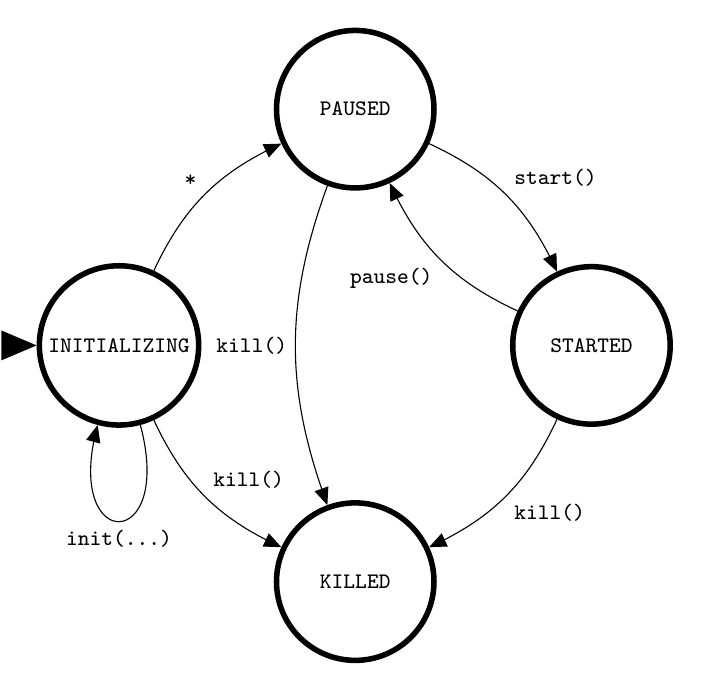
\begin{tikzpicture}[>=triangle 45]\footnotesize
\tikzstyle{state}=[draw=black,circle,line width=2pt,minimum width=2cm]
\node[state] (IN) {\texttt{INITIALIZING}};
\node[state] (PA) at (3,3) {\texttt{PAUSED}};
\node[state] (ST) at (6,0) {\texttt{STARTED}};
\node[state] (KI) at (3,-3) {\texttt{KILLED}};
\draw[->,loop below] (IN) to node[below] {\texttt{init(...)}} (IN);
\draw[->,line width=2pt] (-1.125,0) to (IN);
\draw[->,bend left=20] (IN) to node[above left] {\texttt{*}} (PA);
\draw[->,bend right=20] (IN) to node[above right] {\texttt{kill()}} (KI);
%\draw[->,bend left=20] (PA) to node[below right] {\texttt{RESET}} (IN);
\draw[->,bend left=20] (PA) to node[above right] {\texttt{start()}} (ST);
\draw[->,bend left=20] (ST) to node[below left] {\texttt{pause()}} (PA);
\draw[->,bend left=20] (ST) to node[below right] {\texttt{kill()}} (KI);
\draw[->,bend right=20] (PA) to node[left] {\texttt{kill()}} (KI);
%\draw[->,bend left=20] (ST) to node[below] {\texttt{RESET}} (IN);

\end{tikzpicture}
\caption{Different states of the environment interface and state transitions.}
\caption{FIG:EMS}
\end{figure}


\todo{Write something}

\subsection{Agents and Controllable Entities}

An important concept of \EIS is the separation of concerns, that is the distinction between
1. agents that are software structures that act as percept-processors and action-generators on the platform side,
and 2. controllable entities that are software structures that act as percept-generators and action-processors on the environment side. The connections between agents and controllable entities is made possible by the 
\emph{agents-entities-relation}, that in its essence a subset of the crossproduct of the set of agents and the set of entities. 

The environment-interface in general is very agnostic about the internal structure of both agents and entities, and thus stores them internally only represented as strings (see Fig.~\ref{AGENREL}). These strings are then associated in the agents-entities-relation. How, we will show later. Acting an perceiving is then to be mapped respectively.

\begin{figure}[h]
\begin{center}
\begin{tikzpicture}[line width=2pt,scale=1]\large
\tikzstyle{aeid}=[draw=black,circle, minimum size = 0.75cm, line width=1pt, inner sep=0]
\tikzstyle{object}=[draw=black,circle, minimum size = 1cm, line width=1.5pt, inner sep=0]
\tikzstyle{conn}=[draw=black,line width=1.5pt]
\tikzstyle{connthin}=[draw=black,line width=1pt]

%\draw[-,dashed,line width=1pt] (4,5) to (4,-2.75);
\node(text1) at(0,3.75){\Large APL Side};
\node(text1) at(8.5,3.75){\Large Environment Side};
\node(text1) at(4,3.7){\Large Interface Layer};
\draw[-,dashed,line width=1pt] (2,4) to (2,-2.75);
\draw[-,dashed,line width=1pt] (6,4) to (6,-2.75);

\node[] (ag1) at (0,2) {\bf Agent};
\node[] (ag2) at (0,0) {\bf Agent};
\node[] (ag3) at (0,-2) {\bf Agent};

\node[aeid] (aid1) at (3,1.25) {Id};
\node[aeid] (aid2) at (3,0) {Id};
\node[aeid] (aid3) at (3,-1.25) {Id};

\node[aeid] (eid1) at (5,1.5) {Id};
\node[aeid] (eid2) at (5,0.5) {Id};
\node[aeid] (eid3) at (5,-0.5) {Id};
\node[aeid] (eid4) at (5,-1.5) {Id};

\node[] (en1) at (8,2) {
\includegraphics[width=0.75cm]{robot}};
\node[] (en2) at (8,0.75) {
\includegraphics[width=0.75cm]{robot}};
\node[] (en3) at (8,-0.75) {
\includegraphics[width=0.75cm]{robot}};
\node[] (en4) at (8,-2) {
\includegraphics[width=0.75cm]{robot}};

\draw[conn, bend left=10] (ag1) to (aid1);
\draw[conn] (ag2) to (aid2);
\draw[conn, bend right=10] (ag3) to (aid3);

\draw[conn, bend right=10] (en1) to (eid1);
\draw[conn, bend right=5] (en2) to (eid2);
\draw[conn, bend left=5] (en3) to (eid3);
\draw[conn, bend left=10] (en4) to (eid4);

\draw[connthin] (aid1) to (eid1);
\draw[connthin] (aid2) to (eid2);
\draw[connthin] (aid2) to (eid3);
\draw[connthin] (aid3) to (eid4);

\end{tikzpicture}

\end{center}
\caption{The agent entities-relation. Agents are percept processors and action generators that live on the APL side. Controllable entities are percept generators and action processors and live on the environment side. Both agents and controllable entities are represented via identifiers on the interface layer.}
\label{AGENREL}
\end{figure}



\newpage
\section{EIS PLATFORM GUIDE}

In this section we will provide an tutorial about how to integrate \EIS into your (agent programming) platform. 
We suppose that you have already downloaded the complete package as described earlier. 

\subsection{Linking and Loading}

The first thing that you have to do is adding \EIS to the class-path of your project. We have already described this earlier.
The next thing that you have to do is to employ the jar-loading-mechanism that comes with \EIS. 
Specific environment-interfaces are distributed as jar-files. 
The class \texttt{eis.EILoader} should be used to load an environment-interface from a jar-file and instantiate it.
Use the method \texttt{fromJarFile}:
\begin{verbatim}
EnvironmentInterfaceStandard ei = null;
try {
    ei = EILoader.fromJarFile(new File(jarFileName));
} catch (IOException e) {
    // TODO handle the exception
}
\end{verbatim}
Note that you have to handle exceptions that are potentially thrown by the invocation of the method. 
Possible causes for failure could be that the file does not exist or that the version (\EIS has a versioning-system) does not match the required one.

\subsection{Attaching Listeners for Interface-Platform Communication}

Communication with \EIS-interfaces is facilitated 1. by calling specific methods, and 2. by handling callbacks
that the respective interfaces raise. \EIS provides two listener-interfaces: 
\begin{itemize}
\item \texttt{eis.EnvironmentListener} for handling state changes of the interface, and
\item \texttt{eis.AgentListener} for handling percepts-as-notifications.
\end{itemize}

On the platform side you should provide classes that implement these interfaces.
When you run the system you are supposed to register instances of these classes to the instantiated environment-interface, using these methods of \texttt{eis.EnvironmentInterfaceStandard}:
\begin{itemize}
\item \texttt{attachEnvironmentListener(EnvironmentListener listener)} for attaching an environment-listener, and
\item \texttt{attachAgentListener(AgentListener listener)} for attaching an agent-listener.
\end{itemize}

You can attach as many listeners as you like. Note also, that you can unregister any listener during runtime using these methods:
\begin{itemize}
\item \texttt{detachEnvironmentListener(EnvironmentListener listener)} for detaching an environment-listener, and
\item \texttt{detachAgentListener(AgentListener listener)} for detaching an agent-listener.
\end{itemize}

\subsection{Managing the Environment State}

In order to receive notifications about environment-state changes you have to implement the \texttt{eis.EnvironmentListener} interface and register at least one instance of a respective class via
\texttt{attachEnvironmentListener}. Every time the state changes, the environment-interface will
invoke this method, which you have to implement in order to react to these changes:
\begin{quote}
\texttt{void handleStateChange(EnvironmentState newState);}
\end{quote}
Note that you can query the state at any time by invoking this method of \texttt{eis.EnvironmentInterfaceStandard}:
\begin{quote}
\texttt{EnvironmentState getState();}
\end{quote}

To manipulate the state you have access to this set of methods:
\begin{itemize}
\item\texttt{void init(Map<String,Parameter> parameters) throws ManagementException;}
\item\texttt{void start() throws ManagementException;}
\item\texttt{void pause() throws ManagementException;}
\item\texttt{void kill() throws ManagementException;}
\end{itemize}

You can initialize an environment-interface by calling \texttt{init} with a set of key-value pairs.
Note that all these methods raise a \texttt{ManagementException} in the case that the respective
state transition is not supported. To query whether a state-transition is supported at all you can 
employ this set of methods:
\begin{itemize}
\item\texttt{boolean isInitSupported();} returns \texttt{true} if \texttt{init(...)} is supported,
\item\texttt{boolean isStartSupported();}  returns \texttt{true} if \texttt{start()} is supported,
\item\texttt{boolean isPauseSupported();}  returns \texttt{true} if \texttt{pause()} is supported, and
\item\texttt{boolean isKillSupported();}  returns \texttt{true} if \texttt{kill()} is supported.
\end{itemize}
		
	
\subsection{Setting up Agents, Acting and Perceiving}

register/unregister
acting
allpercepts
notifications

Now that you have successfully instantiated an environment-interface you have to register your agents.
Since \EIS is very agnostic when it comes to the type/structure/architecture of your agents you only have to
register your agents by providing their names. The reason for this is the desired generality. 
So let us assume that you have some agent, which is represented by its name.
You can register the agent like this:
\begin{verbatim}
String agentName = ... ; // the name of your agent
try {
    ei.registerAgent(agentName);
} catch (AgentException e) {
  // TODO handle the exception
}
\end{verbatim}
Again, you have to handle possible exceptions. 
The invocation fails if an agent with the same name has already registered.
You can also unregister an agent if you want to cut it off from the environment-interface:
\begin{verbatim}
try {
    ei.unregisterAgent(agentName);
} catch (AgentException e) {
  // TODO handle the exception
}
\end{verbatim}
Here the invocation fails if the agent has not been registered to the interface.

But why do you have to register your agents to the environment-interface? 
You have to do so because the next thing we are going to do is associating agents with entities.
We differentiate between agents, which we only assume to be software-agents, and controllable entities,
which provide agents with sensory and effectoric capabilities. 
Due to the fact that we do not assume anything about the nature of an environment-interface, we have to
make this distinction. 
Agents act and perceive through entities, entities facilitate the situatedness of agents.
A nice example for an entity is a simulated elevator. 
An agent that controls that elevator-entity can make it move
to a specific floor and perceive its current floor. In order to have an agent control an entity both have to be associated.
Similar to agents, entities are only represented by their name (again a String). 
So assuming that you know that there is an entity with the name \texttt{"car1"}, you can make your agent control it like this:
\begin{verbatim}
try {
    ei.associateEntity(agentName, "car1");
} catch (RelationException e) {
  // TODO handle the exception
}
\end{verbatim}
The invocation could fail, so you have to handle the exception. Note that this a very naive way to associate your agent
with an entity, because it assumes that you know the name of the entity beforehand. 
You can however query the interface for all free entities and associate your agent with the first one:
\begin{verbatim}
LinkedList<String> ens = ei.getFreeEntities();
try {
    ei.associateEntity(agentName, ens.removeFirst());
} catch (RelationException e) {
  // TODO handle the exception
}
\end{verbatim}
Which policy you apply here is your decision. There are more methods for manipulating the agents-entities-relationship
(see the javadoc). Note that you can also query the type of an entity with the method \texttt{getType}. This could be useful
for example if you want to instantiate different types of agents for different types of entities.

Now that you have your agent registered and associated with an entity, or you have already iterated the process and associated
several agents with several entities, you want to make them act and perceive. Acting is quite simple. You have to invoke
the method \texttt{performAction} like this:
\begin{verbatim}
Action action = ... // this has to be an EIS-action
try {
    Vector<Percept> ps = eis.performAction(agentName, action);
} catch (ActException e) {
  // TODO handle the exception
} catch (NoEnvironmentException e) {
  // TODO handle the exception
}
\end{verbatim}
The action must be an instance of \texttt{eis.iilang.Action}. You could for example instantiate an action like this:
\begin{verbatim}
Action action = new Action("goto", new Ident("up"));
\end{verbatim}
It might be necessary to implement a mapping from your definition of what an action is to \EIS-actions.
Note that performing an action could return a percept. This is necessary for active sensing. 
Make sure that such return-values are handled properly.

Note that you can sometimes (depending on the environment-interface) associate a single agent with several entities.
This can be reflected by \texttt{performAction} that accepts an optional array of strings 
(vararg language feature\footnote{\url{http://java.sun.com/developer/JDCTechTips/2005/tt0104.html}}) as the third parameter. 
The array should contain a subset of the set of entities that are associated with the agent: 
\begin{verbatim}
try {
  Vector<Percept> ps = eis.performAction(agentName, action,"entity1","entity2");
} catch (ActException e) {
  // TODO handle the exception
} catch (NoEnvironmentException e) {
  // TODO handle the exception
}
\end{verbatim}
If the array is empty, all
entities will be taken into account. Note that you can determine the source (e.g. the entity) of each percept via the
\texttt{getSource}-method.

You definitely are advised to handle the exceptions. \texttt{NoEnvironmentException} is thrown if the environment-interface
is not properly connected to an environment. \texttt{ActException} is thrown if the action could not be executed. Possible
reasons for that are reflected by the type of the exception:
\begin{verbatim}
try {
  ei.performAction(agentName, action,entities);
} catch (ActException e) {
  if( e.type == NOTYPE ) {
    // TODO handle the exception
  } else if( e.type == NOTREGISTERED ) {
    // TODO handle the exception
  } else if( e.type == NOENTITIES ) {
    // TODO handle the exception
  } else if( e.type == WRONGENTITY ) {
    // TODO handle the exception
  } else if( e.type == WRONGSYNTAX ) {
    // TODO handle the exception
  } else if( e.type == FAILURE ) {
    // TODO handle the exception
  }
} catch(NoEnvironmentException e) {
  // TODO handle the exception
}
\end{verbatim}

The type \texttt{NOTSPECIFIC} denotes that the type of the exception has not been indicated specifically. 
Although we expect  more detailed information about why the method has failed, we do not enforce this.
\texttt{NOTREGISTERED} indicates that the agent has not registered to the environment-interface.
\texttt{NOENTITIES} on the other hand communicates that the agent has no associated entities.
\texttt{WRONGENTITY} denotes that at least one of the provided entities is not associated with the agent.
\texttt{NOTSUPPORTEDBYTYPE} indicates that the type of the entity does not support the execution of the action.
\texttt{WRONGSYNTAX} indicates that the syntax of the action is wrong. 
That is the case when the name of the action is not available and when the parameters do not match (number of parameters or their types and structure).
And \texttt{FAILURE} indicates that the action has failed although it matched all mentioned requirements. 
For example \texttt{goto(up)} could fail if the path is blocked in the respective direction.
 
Now let us talk percepts. There is a method to retrieve all percepts. This has been shown to be very useful for some APL platforms.
You can do this:
\begin{verbatim}
try {
  LinkedList<Percept> percepts = ei.getAllPercepts(agentName);
  // TODO process the percepts
} catch (PerceiveException e) {
  // TODO handle the exception
} catch (NoEnvironmentException e) {
  // TODO handle the exception
}
\end{verbatim}
After the invocation you have to make sure that the percepts are processed in a proper manner. 
Also a \texttt{PerceiveException} is thrown if perception fails, that is if the agent is not registered or has no associated
entities. An instance of \texttt{NoEnvironmentException} is thrown if there is no environment. Similar
to \texttt{performAction} the method \texttt{getAllPercepts} supports a vararg for restricting the call to a subset of the
associated entities.

Now let's talk about the third and final way to get percepts from the environment-interface: percepts-as-notifications.
\EIS supports sending percepts to the agents on special occasions without a request to do so. That is, environments
sending percepts. 
In order to allow your agents to receive such percepts, your platform has to implement the interface \texttt{eis.AgentListener} and its method \texttt{handlePercept(String agent, Percept percept)}. 
Furthermore you have to register the listener to the environment-interface.
The string \texttt{agent} of the \texttt{handlePercept}-method indicates the recipient of the percept \texttt{percept}.
Note that it is your responsibility to make sure that the percept is passed to the respective agent.

You can establish percepts-as-notifications like this:
\begin{verbatim}
class YourPlatform implements AgentListener {

  EnvironmentInterface Standard ei;
  
  ...

  public void init() {
    eis.attachAgentListener(agentName, this);
  }

  public void handlePercept(String agent, Percept percept) {
    // TODO pass the percept to the agent
  }

}
\end{verbatim}

Now we will discuss \emph{environment-events}. Such events are generated if 1. the set of entities changes or is modified, an 2. if the executional-state of the environment changes. Again you have to implement the interface 
\texttt{eis.EnvironmentListener} and its
methods: 
\begin{verbatim}
class YourPlatform implements EnvironmentListener {

  EnvironmentInterface Standard ei;
  
  ...

  public void init() {
    eis.attachEnvironmentListener(this);
  }

  public void handleFreeEntity(String entity) {
    // TODO handle event
  }
  
  public void handleNewEntity(String entity) {
    // TODO handle event
  }
  
  public void handleDeletedEntity(String entity) {
    // TODO handle event
  }
  
  public void handleEnvironmentEvent(EnvironmenEvent event) {
    // TODO handle event
  }

}
\end{verbatim}

The method \texttt{handleNewEntity} is called when there is a new entity, wheras \texttt{handleFreeEntity} is called
when an entity is freed, and \texttt{handleDeletedEntity} is called when an entity is deleted. 
%Do not forget to register the listener to the environment-interface via \texttt{attachEnvironmentListener}.
Again, you have to come up with your own platform-specific policy for new/free/deleted entities. 
We will come back to \texttt{handleEnvironmentEvent} in a minute.

Finally we will discuss methods of environment-management. For managing the environment you can use
the method \texttt{manageEnvironment}:
\begin{verbatim}
EnvironmentCommand command = ...; 
try {
    ei.manageEnvironment(command);
} catch (ManagementException e) {
    // TODO Auto-generated catch block
} catch (NoEnvironmentException e) {
    // TODO Auto-generated catch block
}
\end{verbatim}
An environment-command can either be: starting the environment, killing it, pausing its execution, resetting it, and
initializing it with parameters. A \texttt{ManagementException} is thrown when the command passed as a parameter
is not supported. We do not assume that all environments support all environment-commands (if any at all). 
A \texttt{NoEnvironmentException} is thrown when the environment-interface is not connected to an environment.

The environment-interface can also notify about the change of the state of the execution of the environment.
Such an event can either be that the environment has been started, killed, paused, reset, or initialized.
Note that we do not assume that all environment-interfaces notify about such events.



\newpage
\section{EIS INTERFACE GUIDE}

The purpose of this section is to explain how you can make an environment \EIS-compatible. 
Essentially there are two solutions to that problem:
\begin{enumerate}
\item implementing the Java-interface \texttt{apleis.EnvironmentInterfaceStandard}, or
\item extending the abstract class \texttt{apleis.EIDefaultImpl}.
\end{enumerate}

We usually suggest that extending the abstract-class is way-to-go, because the default-implementation
already provides a lot of the functionality that is required from each specific environment interface.
Most of the functionality, which comes as a couple of methods, can be overridden and thus changed
according to the needs of the developer.

In the following we will explain the basic mechanisms of \EIS, that is
\begin{itemize}
\item associating agents and entities,
\item acting and perceiving,
\item environment state management, and
\item querying functionality.
\end{itemize}

TODO both ways

\subsection{General Issues}

listeners!

\subsection{Agents and Entities}

managing the agents-entities-relation


\subsection{Acting and Perceiving}

\begin{quote}
\texttt{Map<String,Percept> performAction(String agent, Action action,
			String... entities) throws ActException;}
\end{quote}

This method yields an exception if the execution of the provided action fails. 
This exception is an instance of \texttt{eis.exceptions.ActException} and its 
\texttt{type}-field denotes the reason for the failure. Values are:
\begin{itemize}
\item\texttt{NOTSPECIFIC}: if there is no specific reason for the failure (this type should be avoided).
\item\texttt{NOTREGISTERED}: if the agent is not registered.
\item\texttt{NOENTITIES}: if the agent as no associated entities and thus cannot act.
\item\texttt{WRONGENTITY}: if the array \texttt{entities} contains at least one entity that is not associated with the agent.
\item\texttt{NOTSUPPORTEDBYENVIRONMENT}: if the action is not supported by the environment.
\item\texttt{NOTSUPPORTEDBYTYPE}: if the action is not supported by the type of an entity.
\item\texttt{NOTSUPPORTEDBYENTITY}: if the action is not supported by the entity itself.
\texttt{FAILURE}: if the action is supported by the execution fails. 
\end{itemize}
\todo{maybe examples for failures}

When implementing the \texttt{EnvironmentInterfaceStandard} interface you have to make sure that your
implementation of�\texttt{performAction} fits the specification above when it comes to the exception-types.

The \texttt{EIDefaultImpl} on the other hand already enforces the specification and requires you to implement a set of helper methods:
\begin{itemize}
\item\texttt{boolean isSupportedByEnvironment(Action action)}: is supposed to return \texttt{true} iff the action
is supported by the environment.
\item\texttt{boolean isSupportedByType(Action action, String type)}: is supposed to return \texttt{true} iff the action
is supported by the entity-type.
\item\texttt{boolean isSupportedByEntity(Action action, String entity)}: is supposed to return \texttt{true} iff the action
is supported by the entity.
\item\texttt{Percept performEntityAction(String entity, Action action) throws ActException}: is supposed to execute the
action or trigger its execution in the environment. On top of that it is expected that an \texttt{ActException} with type
\texttt{FAILURE} is thrown if the action fails to execute.
\end{itemize}

The implementation of \texttt{performAction} in \texttt{EIDefaultImpl} works as follows:
\begin{enumerate}
\item if \texttt{agent} is not registered throw an \texttt{ActException} with type \texttt{NOTREGISTERED},
\item if \texttt{agent} has no associated entities throw an \texttt{ActException} with type \texttt{NOENTITIES},
\item if \texttt{entities} contains at least one entity that is not associated with \texttt{agent} throw an \texttt{ActException} with type \texttt{WRONGENTITY},
\item if \texttt{isSupportedByEnvironment(...)} returns \texttt{false} 
throw an \texttt{ActException} with type \texttt{NOSUPPORTEDBYENVIRONMENTs},
\item \texttt{isSupportedByType(...)} returns \texttt{false} for at least one type of the entities
throw an \texttt{ActException} with type \texttt{NOSUPPORTEDBYTYPE},
\item if \texttt{isSupportedByEntity(...)} returns \texttt{false} for at least one entity in \texttt{entities} 
throw an \texttt{ActException} with type \texttt{NOSUPPORTEDBYENTITY},
\item call \texttt{performEntityAction(...)} which can yield an \texttt{ActException} with type \texttt{FAILED}, which is then rethrown.
\end{enumerate}



	
\subsection{Querying Mechanism}

\begin{verbatim}
default implementation versus interface-definition
  interface comes without any functionality
versioning
associating agents with entities
environment management support
  TODO copy EMS-stuff here
acting and perceiving
action validation mechanism
  explain act exception
  using interface: make sure that the exceptions are instantiated the right way
  using default impl... implement the isSupported etc methods
  act-exception: interface vs defaultimpl
querying-mechanism
  query the interface in general
  query entities in specific
footnotes: what is new/different in EIS 0.3
checklists?
\end{verbatim}










\end{document}

\section{Integration}



\section{Included environment-interfaces}

Wherein we elaborate on environment-interfaces that are included in the \EIS-package.

\subsection{Agent Contest Connector 2007}

In order to run the contest environment you have to download the package including the MASSim-server from
the Multi-Agent Contest homepage\footnote{\url{http://www.multiagentcontest.org}}. 

\medskip\noindent{\textbf{Environment description:}} the environment is a grid-like, partially-accessible world. Goldminers. The goal is to collect as much gold as possible. More information is available at the 
contest homepage.

\medskip\noindent{\textbf{Jar-file:}} \texttt{eis-acconnector2007-0.2.jar} (included in the \EIS-package).

\medskip\noindent{\textbf{Entities:}}
\begin{description}
\item[\texttt{connector1},$\ldots$,\texttt{connector6}] each one is a connector to a single goldminer in the environment.
\end{description}

\noindent{\textbf{Types of entities:}} this interface does not take into account different types of entities.

\medskip\noindent{\textbf{Actions:}}
\begin{description}
\item[\texttt{connect(Identifier, Numeral , Identifier, Identifier)}] connects to the MASSim-server.
The first identifier is the hostname of the server. The numeral is its port. The second identifier denotes the user-name,
the final one denotes the password. This action has to be performed successfully in order to allow for other actions.
Example: \texttt{connect("139.174.100.201",12300,"agentred1","dfkj39")}.
\item[\texttt{skip}] has no effect.
\item[\texttt{right}] moves the goldminer to the right.
\item[\texttt{up}] moves the goldminer up.
\item[\texttt{left}] moves the goldminer left.
\item[\texttt{down}] moves the goldminer down.
\item[\texttt{pick}] picks up gold.
\item[\texttt{drop}] drops gold.
\item[\texttt{mark(Identifier)}] marks the current cell with a string.
\item[\texttt{unmark}] unmarks the current cell.

\end{description}

\noindent{\textbf{Percepts:}} all those percepts are both propagated as notifications and returned by the
\texttt{getAllPercepts}-method. Note that the interface implements a queue of percepts that is filled every time
a message from the MASSim-server is received and whose first entry is retrieved every time the \texttt{getAllPercepts}-method is called. The interface does not hold a world-model.
\begin{description}
\item[\texttt{connectionLost}] indicates that the connection to the server has been lost. 
\item[\texttt{simStart}] indicates that the simulation has begun.
\item[\texttt{corralPos(Numeral, Numeral, Numeral, Numeral)}] is the position of the corral the first two numbers indicate the upper-left- 
the last two ones indicate the lower-right-corner. Example: \texttt{corralPos(1,1,10,10)}.
\item[\texttt{gridSize(Numeral, Numeral)}] represents the size of the grid. The first value is the width, the second one is 
the height. Example:\texttt{gridSize(100,100)}.
\item[\texttt{simId(Identifier id)}] denotes the id of the simulation. Example: \texttt{simId("cowSkullMountain")}
\item[\texttt{lineOfSight(Numeral num)}] indicates how far the respective entity can see. 
Example: \texttt{lineOfSight(8)}
\item[\texttt{opponent(Numeral name)}] denotes the opponent in the current match. 
Example: \texttt{opponent("StampedeTeam")}
\item[\texttt{steps(Numeral num)}] indicates how many steps the simulation lasts. Example: \texttt{steps(1000)}
\item[\texttt{simEnd}] indicates that the current simulation is over.
\item[\texttt{result(Identifier)}] represents the result of the simulation. Values could be either \texttt{win},  
\texttt{lose}, or  \texttt{draw}. Example: \texttt{result(win)}
\item[\texttt{finalScore(Numeral)}] represents the final-score of the simulation. Example: \texttt{finalScore(42)}
\item[\texttt{bye}] indicates that the overall tournament is over.
\item[\texttt{cell(Numeral, Numeral, Identifier)}] denote the content of a cell. The numerals represent the position 
relative to the cowboy's current position. The identifier represents the object. 
Possible values are \texttt{agentally}, \texttt{agentenemy}, \texttt{switch}, \texttt{fenceopen}, 
\texttt{fenceclosed}, \texttt{cow}, \texttt{obstacle}, \texttt{empty}, and \texttt{unknown}. 
Example: \texttt{cell(-1,-1,cow)}
%\item[\texttt{id(Numeral num)}] indicates the identifier of the \texttt{id(70)}
\item[\texttt{pos(Numeral x, Numeral y)}] denotes the current position of the cowboy. Example: \texttt{pos(10,15)}
\item[\texttt{currentScore(Numeral)}] denotes the current score. Example: \texttt{currentScore(24)}
\item[\texttt{currentStep(Numeral num)}] indicates the current step of the simulation.
Example: \texttt{currentStep(123)}
\end{description}

\noindent{\textbf{Environment-management:}} not supported.

\subsection{Agent Contest Connector 2009}

In order to run the contest environment you have to download the package including the MASSim-server from
the Multi-Agent Contest homepage\footnote{\url{http://www.multiagentcontest.org}}. 

\medskip\noindent{\textbf{Environment description:}} the environment is a grid-like, partially-accessible world. Cowboys are steered
by agents. The goal is to push cows into a corral by frightening them. More information is available at the 
contest homepage.

\medskip\noindent{\textbf{Jar-file:}} \texttt{eis-acconnector2009-0.2.jar} (included in the \EIS-package).

\medskip\noindent{\textbf{Entities:}}
\begin{description}
\item[\texttt{connector1},$\ldots$,\texttt{connector10}] each one is a connector to a single cowboy in the environment.
\end{description}

\noindent{\textbf{Types of entities:}} this interface does not take into account different types of entities.

\medskip\noindent{\textbf{Actions:}}
\begin{description}
\item[\texttt{connect(Identifier, Numeral , Identifier, Identifier)}] connects to the MASSim-server.
The first identifier is the hostname of the server. The numeral is its port. The second identifier denotes the user-name,
the final one denotes the password. This action has to be performed successfully in order to allow for other actions.
Example: \texttt{connect("139.174.100.201",12300,"agentred1","dfkj39")}.
\item[\texttt{move(Identifier direction)}] moves the cowboy to a specified direction. 
Possible actions are \texttt{north}, \texttt{northeast}, \texttt{east}, \texttt{southeast}, \texttt{south}, \texttt{southwest},
\texttt{west}, and \texttt{northwest}. Example \texttt{move(east)}
\item[\texttt{skip}] has no effect.
\end{description}

\noindent{\textbf{Percepts:}} all those percepts are both propagated as notifications and returned by the
\texttt{getAllPercepts}-method. Note that the interface implements a queue of percepts that is filled every time
a message from the MASSim-server is received and whose first entry is retrieved every time the \texttt{getAllPercepts}-method is called. The interface does not hold a world-model.
\begin{description}
\item[\texttt{connectionLost}] indicates that the connection to the server has been lost. 
\item[\texttt{simStart}] indicates that the simulation has begun.
\item[\texttt{corralPos(Numeral, Numeral, Numeral, Numeral)}] is the position of the corral the first two numbers indicate the upper-left- 
the last two ones indicate the lower-right-corner. Example: \texttt{corralPos(1,1,10,10)}.
\item[\texttt{gridSize(Numeral, Numeral)}] represents the size of the grid. The first value is the width, the second one is 
the height. Example:\texttt{gridSize(100,100)}.
\item[\texttt{simId(Identifier id)}] denotes the id of the simulation. Example: \texttt{simId("cowSkullMountain")}
\item[\texttt{lineOfSight(Numeral num)}] indicates how far the respective entity can see. 
Example: \texttt{lineOfSight(8)}
\item[\texttt{opponent(Numeral name)}] denotes the opponent in the current match. 
Example: \texttt{opponent("StampedeTeam")}
\item[\texttt{steps(Numeral num)}] indicates how many steps the simulation lasts. Example: \texttt{steps(1000)}
\item[\texttt{simEnd}] indicates that the current simulation is over.
\item[\texttt{result(Identifier)}] represents the result of the simulation. Values could be either \texttt{win},  
\texttt{lose}, or  \texttt{draw}. Example: \texttt{result(win)}
\item[\texttt{finalScore(Numeral)}] represents the final-score of the simulation. Example: \texttt{finalScore(42)}
\item[\texttt{bye}] indicates that the overall tournament is over.
\item[\texttt{cell(Numeral, Numeral, Identifier)}] denote the content of a cell. The numerals represent the position 
relative to the cowboy's current position. The identifier represents the object. 
Possible values are \texttt{agentally}, \texttt{agentenemy}, \texttt{switch}, \texttt{fenceopen}, 
\texttt{fenceclosed}, \texttt{cow}, \texttt{obstacle}, \texttt{empty}, and \texttt{unknown}. 
Example: \texttt{cell(-1,-1,cow)}
%\item[\texttt{id(Numeral num)}] indicates the identifier of the \texttt{id(70)}
\item[\texttt{pos(Numeral x, Numeral y)}] denotes the current position of the cowboy. Example: \texttt{pos(10,15)}
\item[\texttt{currentScore(Numeral)}] denotes the current score. Example: \texttt{currentScore(24)}
\item[\texttt{currentStep(Numeral num)}] indicates the current step of the simulation.
Example: \texttt{currentStep(123)}
\end{description}

\noindent{\textbf{Environment-management:}} not supported.
\subsection{Carriage Example}

\medskip\noindent{\textbf{Environment description:}} there is a carriage on a circular-track. That track has three 
distinct locations for the carriage two be on. On each side of the carriage is a robot. Both robots can push the carriage.
The environment evolves in a step-wise manner.

\medskip\noindent{\textbf{Jar-file:}} \texttt{eis-carriage-0.2.jar} (included in the \EIS-package).

\medskip\noindent{\textbf{Entities:}}
\begin{description}
\item[\texttt{robot1},\texttt{robot2}] are the two robots in the environment.
\end{description}

\noindent{\textbf{Types of entities:}} this interface does not take into account different types of entities.

\medskip\noindent{\textbf{Actions:}}
\begin{description}
\item[\texttt{push}] pushes the carriage. If both robots push at the same time, the carriage will not move. If only
one robot pushes the carriage will.
\item[\texttt{wait}] has no effect.
\end{description}

\noindent{\textbf{Percepts:}}
\begin{description}
\item[\texttt{step}] indicates that current step of the environment. Propagates via notifications 
\item[\texttt{currentPos(Number)}] denotes the current position of the carriage, either \texttt{0}, \texttt{1}, or \texttt{2}.
Returned by \texttt{getAllEntities}.
\end{description}

\noindent{\textbf{Environment-management:}} not supported.

%\appendix
%\section{EIS-Platform-Integration Checklist}
%\begin{itemize}
%\item[$\square$] add EIS to the class-path of your project
%\item[$\square$] retrieve an environment-interface-jar-file
%\item[$\square$] load environment-interface with \texttt{EILoader}
%\item[$\square$] register your agents
%\item[$\square$] associate your agents with entities provided by the interface
%\item[$\square$] act ant perceive
%\item[$\square$] environment-listening
%\end{itemize}

\end{document}\documentclass[a4]{article}

\usepackage{fullpage}
\usepackage{graphicx}
\usepackage{tikz}
\usepackage{listings}
\usepackage{theorem}
\usepackage{url}
\usepackage{xspace}

\newcommand{\todo}[1]{{\bf [TODO: }\textit{#1}{\bf ]}}
\newcommand{\remark}[1]{{\bf [RemarkKVH: }\textit{#1}{\bf ]}}
\newcommand{\remarktmb}[1]{{\bf [RemarkTMB: }\textit{#1}{\bf ]}}

\newcommand{\EIS}{\textsf{EIS}\xspace}

\newcommand{\Goal}{\textsc{GOAL}\xspace}
\newcommand{\Jason}{\textsc{Jason}\xspace}
\newcommand{\twoAPL}{\textsc{2APL}\xspace}
\newcommand{\Jadex}{\textsc{Jadex}\xspace}

\newtheorem{example}{Example}





\begin{document}


\title{Environment Interface Standard for Agent-Oriented Programming \\
\textit{Environment Interface Implementation Guide for EIS v0.2}
}

\author{Tristan M. Behrens}
\date{\today}

\maketitle

\section{Introduction}

This document's intent is to provide a tutorial for creating environment interfaces for arbitrary environments.
Also it provides a template for documenting your environment-interfaces when making them available.

\section{Environment Interface Implementation Guide}

We would like to coin a new term: \emph{EISification} is the process of taking a given environment, adapting it
to support the Environment Interface Standard, and distributing the result.

The overall GOAL is to take your environment (let it be some already existing one or one that has to be developed),
EISify it and then deploy it as a jar-file, for others to use it. EISification means creating an environment-interface-class
-- this is the \emph{main-class} -- that wraps your environment or connects to it.

These are the essential steps:
\begin{enumerate}
\item set up your project and add \EIS to the class-path. The current version contained in \texttt{eis-0.2-lib.jar}.
\item create the main-class that either implements the standard-interface (\texttt{eis.EnvironmentInterfaceStandard})  
\textbf{or} extends the default-implementation (\texttt{eis.EIDefaultImpl}). 
\item create a jar-file from your classes and specify the main-class in the manifest-file.
\item make the jar-file available.
\end{enumerate}

We recommend using the default-implementation over using the standard-interface.

You can add the jar-file to the class-path directly:
Alternatively, if your project supports  
Maven\footnote{http://maven.apache.org/}, you can add \EIS as a dependency to your \texttt{pom.xml}:
\begin{verbatim}
<dependencies>
  <dependency>
    <groupId>apleis</groupId> 
    <artifactId>eis</artifactId> 
    <version>0.2</version> 
    <scope>compile</scope>
  </dependency>
  ...
</dependencies>
\end{verbatim}


\subsection{Using the default-implementation}

The first thing you would do is create your main-class and let it extend class \texttt{eis.EIDefaultImpl}:
\begin{verbatim}
package yourproject;

import eis.*;

public class MyEnvironmentInterface extends EIDefaultImpl {
  // TODO implement the abstract methods
}
\end{verbatim}
The default-implementation already implements all needed functions. 
You only have to implement methods that are specific to your environment-interface. 

You have to implement the abstract method \texttt{isConnected}:
\begin{verbatim}
public boolean isConnected() {
  // TODO implement
}
\end{verbatim}
This method is supposed to return \texttt{true} if the environment is connected to the environment-interface and \texttt{false}
otherwise. 

Also you have to implement \texttt{getAllPerceptsFromEntity}:
\begin{verbatim}
public LinkedList<Percept> getAllPerceptsFromEntity(String entity) 
    throws PerceiveException, NoEnvironmentException {
  // TODO implement
}
\end{verbatim}
This method should return all percepts of the entity \texttt{entity}.

Also, you should employ percepts-as-notifications wherever possible. Such percepts are supposed to be sent to
agents via instances of \texttt{eis.AgentListener} that have been registered to the interface via its \texttt{attachAgentListener}-method. The default implementation provides the method \texttt{notifyAgents} that allow you 
to send a percept to one, several, or all agents. And the method \texttt{notifyAgentsViaEntity} allows for sending
percepts to all agents that are associated to one, several or all entities.

Now we have to discuss the definition and executions of actions. 
For each action with a fixed named and fixed parameters you have to implement a method.
For example assume that you have a \texttt{goto}-action with a parameter that determines the
direction you would implement:
\begin{verbatim}
public Percept actiongoto(String entity, Ident dir) throws ActException, 
    NoEnvironmentException {
  // TODO implement
}
\end{verbatim}
Note that this is a convention. The action-name itself is mapped to a method-call via Java-reflection.
However if you prefer your own custom mechanism for executing actions feel free to overwrite the \texttt{performAction}-method. 

Before discussing other methods, we have to say something about the exceptions that can be thrown in the likely event
that an action fails. An instance of \texttt{NoEnvironmentException} should be thrown if the environment-interface is not
connected to an environment. If there is a connection an instance of \texttt{ActException} should be thrown. 
Please heed that that exception-class is typed, that is it communicates more detailed information about the 
action-failure by carrying a type that can be queried when the exception is caught. Do it like this:
\begin{verbatim}
// the syntax of the action is wrong
throw new ActException( ActException.WRONGSYNTAX );
\end{verbatim}
The type \texttt{NOTSPECIFIC} is the default type of \texttt{ActException}. We strongly discourage you from using this one.
We expect you to provide more detailed information about why the method has failed.
\texttt{NOTREGISTERED} indicates that the agent has not registered to the environment-interface.
\texttt{NOENTITIES} on the other hand communicates that the agent has no associated entities.
\texttt{WRONGENTITY} denotes that at least one of the provided entities is not associated with the agent.
\texttt{NOTSUPPORTEDBYTYPE} indicates that the type of the entity does not support the execution of the action.
\texttt{WRONGSYNTAX} indicates that the syntax of the action is wrong. 
That is the case when the name of the action is not available and when the parameters do not match (number of parameters or their types and structure).
And \texttt{FAILURE} indicates that the action has failed although it matched all mentioned requirements. 
For example \texttt{goto(up)} could fail if the path is blocked in the respective direction.

The next method is \texttt{release} which is supposed to disconnect the environment-interface from the environment:
\begin{verbatim}
public void release() {
    // TODO release the environment
}
\end{verbatim}
After invoking that method \texttt{isConnected} should always return \texttt{false}.

Finally, let us discuss managing the environment. You should allow for managing the environment by implementing
the method \texttt{manageEnvironment}:
\begin{verbatim}
public void manageEnvironment(EnvironmentCommand command)
        throws ManagementException {
    // TODO implement environment-management	
}
\end{verbatim}
An environment-command can either be: starting the environment, killing it, pausing its execution, resetting it, and
initializing it with parameters. A \texttt{ManagementException} is thrown when the command passed as a parameter
is not supported. We explicitly do note make obligatory that you should implement all environment-commands. If your
environment for example does not support being paused than you do not have to implement the respective commands.
A \texttt{NoEnvironmentException} is thrown when the environment-interface is not connected to an environment.

\subsection{Using the interface}

Instead of extending the default-implementation you can also implement the standard-interface.
The first thing you would do is create your main-class and let it implement the interface \texttt{EnvironmentInterfaceStandard}:
\begin{verbatim}
package yourproject;

import eis.*;

public class MyEnvironmentInterface implements EnvironmentInterfaceStandard {

}
\end{verbatim}
This is of course not everything. You have to implement the interface's methods. Quite some of them, to be honest.
Please have a look at the default-implementation for some inspiration about how to implement those.

The first thing you should do is attaching and detaching environment- and agent-listeners. 
We assume that you internally store a list of registered listeners. For example you could use like in the default implementation
\texttt{Vector<EnvironmentListener>} and \texttt{ConcurrentHashMap<String,HashSet<AgentListener>>} respectively. 
But feel free to use anything that fits your needs
Environment-listeners are used to inform observers about the change of the state of execution of the environment.
Every observer that is interested in such events should register via:
\begin{verbatim}
public void attachEnvironmentListener(EnvironmentListener listener) {
  // TODO store the listener internally
}
\end{verbatim}

It should also be possible to remove an observer:
\begin{verbatim}
public void detachEnvironmentListener(EnvironmentListener listener) {
  // TODO remove the listener from the internal representation
}
\end{verbatim}

For the agent-listeners it is almost the same. 
These are used to send percepts-as-notifications to the agents.
Here you should store for each agent a set of listeners:
\begin{verbatim}
public void attachAgentListener(String agent, AgentListener listener) {
  // TODO store the listener internally
}
\end{verbatim}

Again, removing the listener should also be allowed:
\begin{verbatim}
public void detachAgentListener(String agent, AgentListener listener) {
  // TODO remove the listener from the internal representation
}
\end{verbatim}

Of course when implementing your specialized interface you should implement means to notify the listeners.
Employ agent-listeners to send percepts to agents, and use environment-listeners to send environment events.
Compare with the \texttt{notify*}-methods of the default implementation.

After that you should provide functionality that allow for (un)registering and unregistering agents, and for
(dis)associating agents with entities. To begin it would be good to set-up an internal list of agents, another one for entities,
and some map for associating agents and entities.
For example you could use \texttt{LinkedList<String>} for the lists and \texttt{ConcurrentHashMap<String,HashSet<String>>} for the mapping.

Please allow for registering agents:
\begin{verbatim}
public void registerAgent(String agent) throws AgentException {
  // TODO store internally
}
\end{verbatim}
You should throw an \texttt{AgentException} if the agent has already registered.

Then allow for unregistering:
\begin{verbatim}
public void unregisterAgent(String agent) throws AgentException {
  // TODO remove form internal representation
}
\end{verbatim}
Here you should throw an \texttt{AgentException} if the agent has not registered.

Also make sure that the list of agents can be retrieved:
\begin{verbatim}
public LinkedList<String> getAgents() {
  // TODO return the list of agents
}
\end{verbatim}

And make sure to to the same for entities as well:
\begin{verbatim}
public LinkedList<String> getEntities() {
  // TODO return the list of entities
}
\end{verbatim}

Then associate an agent with an entity
\begin{verbatim}
public void associateEntity(String agent, String entity) throws RelationException {
  // TODO update the mapping
}
\end{verbatim}
Make sure to throw an \texttt{RelationException} if associating the agent with the entity is not possible.
This is the case for example when the agent or the entity are not stored in the internal lists. 

After that allow for freeing an entity from all associations with agents:
\begin{verbatim}
public void freeEntity(String entity) throws RelationException {
  // TODO update the mapping
}
\end{verbatim}
Here you should throw an \texttt{RelationException} if the entity could not be freed. 
That is when is not contained in the internal list of entities.

Do the same for an agent:
\begin{verbatim}
public void freeAgent(String agent) throws RelationException {
    // TODO update the mapping
}
\end{verbatim}

Then remove a specific agent-entity-pair from the mapping:
\begin{verbatim}
public void freePair(String agent, String entity) throws RelationException {
  // TODO update the mapping
}
\end{verbatim}
Again throw an \texttt{RelationException} if the operation fails.

After manipulating the agents-entities-relation it would be useful to allow for querying the data-structures.
You should provide a method that returns the entities associated to an agent:
\begin{verbatim}
public HashSet<String> getAssociatedEntities(String agent) throws AgentException {
}
\end{verbatim}
Make sure to throw an \texttt{AgentException} if the agent is not registered to the interface.

And you should provide the same for an entity:
\begin{verbatim}
public HashSet<String> getAssociatedAgents(String entity) throws EntityException {
}
\end{verbatim}
Here you should throw an \texttt{EntityException} if the entity has not been added to the interface.

Finally return the list of free entities, that is a list of entities that are not associated:
\begin{verbatim}
public LinkedList<String> getFreeEntities() {
}
\end{verbatim}

Also it is necessary to return the type of an entity:
\begin{verbatim}
public String getType(String entity) throws EntityException
\end{verbatim}
Throw an \texttt{EntityException} if the entity does not exist.

Now we have to discuss acting and perceiving. Entities are the ones that provide agents with sensory and effectoric
capabilities. Agents act and perceive through entities.

This is the first essential method:
\begin{verbatim}
public LinkedList<Percept> performAction(String agent, Action action, String...entities)
	throws ActException, NoEnvironmentException {
  // TODO perform the action and return a percept
}
\end{verbatim}
It should allow an agent to act through a set of his associated entities provided as an array. If the array is empty
all associated entities should perform the action. Here you need to throw an \texttt{ActException} if the action
fails, that is when one or more of the entities failed to execute the action or of one or several of the provided
entities are not associated. And you need to throw an \texttt{NoEnvironmentException} of the environment-interface
is not connected to an environment. Note that the return-value is also interesting. The method can also be used
to facilitate active-sensing. Some actions might just return something simple like a \texttt{"success"}-Percept or 
something very sophisticated. Finally you should make sure to indicate the origin-entity of each percept via
the \texttt{setSource}-method of \texttt{Percept}.

You should also implement this method for retrieving all percepts:
\begin{verbatim}
public LinkedList<Percept> getAllPercepts(String agent, String...entities) 
    throws PerceiveException, NoEnvironmentException {
  // TODO return all percepts   
}
\end{verbatim}
This method is supposed to return all percepts of the entities that are associated with an agent. 
Again the associated entities are provided as an array. If the array is empty all entities are used for sensing.
The method fails with an \texttt{PerceiveException} if perceiving through one or several entities is not possible,
or of one or several of the provided entities are not associated. The \texttt{NoEnvironmentException} is thrown
if no environment is connected.


\begin{verbatim}
      what happens once you implement the interface? what do you have to do?
        you have to implement a couple of methods
          isConnected
          manageEnvironment
          release
      what is which method supposed to do?
\end{verbatim}

\section{Environment Interface Documentation Policy}

In order to ensure transparency and accessibility when publishing your environment-interfaces, you should
provide a documentation. That documentation should contain all necessary information, including 
1. a description of the environment, 
2. the name of the jar-file that contains the environment-interface,
3. the names of the entities that populate the environment,
4. the types of those entities,
5. the actions of the entities, and
6. the percepts.

Please provide a description of the environment:\smallskip\\
\fbox{\begin{minipage}{15cm}
\textbf{Environment description:} the environment is a simple 3-dimensional world with a ground level. It is populated
by jeeps that are not controllable entities. Controllable entities are unmanned vehicles, that should be used to locate
the jeeps.
\end{minipage}}\medskip

After that you should say, in which jar-file the environment-interface is contained, and optionally where to find that file:\smallskip\\
\fbox{\begin{minipage}{15cm}
\textbf{Jar-file:} \texttt{uv-simulation.jar}
\end{minipage}}\medskip

Now you should give an overview of the different entities that populate the environment. Please provide their names
and their characteristics:\smallskip\\
\fbox{\begin{minipage}{15cm}
\textbf{Entities:}
\begin{description}
\item[\texttt{uv1},\texttt{uv2},$\ldots$] are several unmanned ground vehicles. There are 100 in the simulation.
\end{description}
\end{minipage}}\medskip

Please provide the types of entities as well:\smallskip\\
\fbox{\begin{minipage}{15cm}
\begin{description}
\item[\texttt{groundvehicle}] these are unmanned ground vehicles.
\item[\texttt{airvehicle}] these are unmanned aerial vehicles.
\end{description}
\end{minipage}}\medskip

Now, denote and describe the different actions that are supported. Please make sure to include the parameters
of the actions and their meaning. And do not forget to mention, what kind of percepts an action would return,
if it was a sensing action\smallskip\\
\fbox{\begin{minipage}{15cm}
\textbf{Actions:}
\begin{description}
\item[\texttt{move(Identifier)}] moves the entity into a specific direction. Possible directions are:
\texttt{north}, \texttt{east}, \texttt{south}, and \texttt{west}. Example: \texttt{move(east)}
\item[\texttt{useCamera}] uses the camera and returns the most prominent, visible object.
\item[\texttt{liftOff}] lifts an entity off the ground. Only available to aerial vehicles.
\item[\texttt{land}] lands and entity. Only available to aerial vehicles.
\end{description}
\end{minipage}}\medskip

Now describe the different percepts. Again please describe the possible parameters and their meaning. Also
explain how the different percepts are made available. Do you retrieve an agent via the \texttt{getAllPercepts}-method,
by a notification, or by both?\smallskip\\
\fbox{\begin{minipage}{15cm}
\textbf{Percepts:}
\begin{description}
\item[\texttt{time(Numeral)}] indicates the current time-stamp of the simulation. Returned by \texttt{getAllPercepts}
and send as a notification every second. 
\item[\texttt{currentPos(Number,Number,Number)}] denotes the current position of the vehicle in the three dimensions of
space. Returned by \texttt{getAllPercepts} and send as a notification every second.
\end{description}
\end{minipage}}\medskip

And finally make clear, which means for environment-management are supported:\smallskip\\
\fbox{\begin{minipage}{15cm}
\textbf{Environment-management:} the environment can be initialized with a parameter that denotes that map
that should be used. All other environment-commands are not supported.
\end{minipage}}\medskip




\end{document}